\documentclass[../report.tex]{subfiles}

\begin{document}

\chapter{Results} % Performance comparison for the KHAPE library (not the password manager use case).
 


\section{KHAPE endpoints} % What endpoint take the most time during auth and register ? 
% 2 boite à moustache (en mode histogram), x = each endpoint, y = time
% \pgfplotsset{width=\textwidth, height=6cm}

\subsection*{Registration}

\pgfplotsset{width=\textwidth-1.1cm}

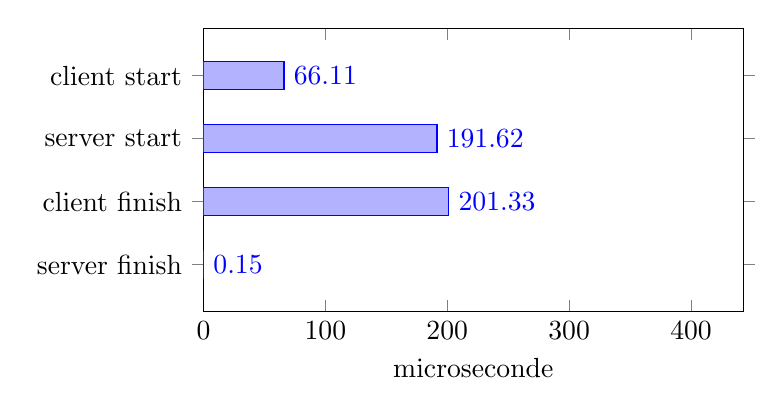
\begin{tikzpicture}
\begin{axis}[
    xbar,
    y=0.8cm,
    xmin=0, xmax=385,
    enlarge y limits=0.25,
    enlarge x limits={0.15, upper},
    legend style={at={(0.5,-0.2)},
    anchor=north,legend columns=-1},
    xlabel={microseconde},
    symbolic y coords={server finish, client finish, server start, client start},
    ytick=data,
    nodes near coords,
    nodes near coords align={horizontal},
]
\addplot coordinates {
    (0.15336,server finish)
    (201.33,client finish)
    (191.62,server start)
    (66.105,client start)
};
\end{axis}
\end{tikzpicture}


\subsection*{Authentication}

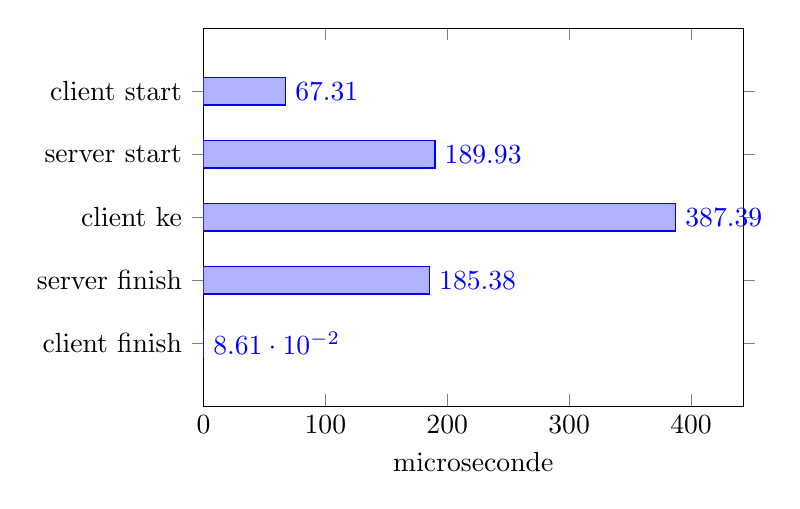
\begin{tikzpicture}
\begin{axis}[
    xbar,
    y=0.8cm,
    xmin=0, xmax=385,
    enlarge y limits=0.25,
    enlarge x limits={0.15, upper},
    legend style={at={(0.5,-0.2)},
    anchor=north,legend columns=-1},
    xlabel={microseconde},
    symbolic y coords={client finish, server finish, client ke, server start, client start},
    ytick=data,
    nodes near coords,
    nodes near coords align={horizontal},
]
\addplot coordinates {
    (0.086069,client finish)
    (185.38,server finish)
    (387.39,client ke)
    (189.93,server start)
    (67.308,client start)
};
\end{axis}
\end{tikzpicture}



\subsection{Ideal Cipher vs AES} % isolated, endpoints, overall. How does it change the performance of each endpoint and overall ?
% 2 boite à moustache (en mode histogram), x = each endpoint, y = time. Comparison with the standard time (above)

\subsection{With OPRF vs without OPRF} % endpoints, overall. How does it change the performance of each endpoint and overall ?
% 2 boite à moustache (en mode histogram), x = each endpoint, y = time. Comparison with the standard time (above)

\subsection{With SlowHash vs without SlowHash} % endpoints, overall. How does it change the performance of each endpoint and overall ?
% 2 boite à moustache (en mode histogram), x = each endpoint, y = time. Comparison with the standard time (above)


\section{(OPAQUE endpoints)} % same as KHAPE endpoints. Shows default parameters and similar parameters as KHAPE


\section{OPAQUE vs KHAPE} % endpoints, overall. How does KHAPE performance compare to OPAQUE with ~same~ parameters (OPRF, no SlowHash, same curve ?, same hash ?)
% 2 histogram, one for auth overall, one for register overall, x = OPAQUE(default) OPAQUE(same params) KHAPE(IC OPRF) KHAPE(IC noOPRF) KHAPE(AES OPRF) KHAPE(AES noOPRF), y = time. Each histogram bar is separated in another color to show each endpoint proportion
% highlight the 2 bar where OPAQUE and KHAPE have the same params, put the rest aside (just for info)


\section{Input size} % Does the uid and password size has any inpact on the performance of auth and register ?

\section{Message size}

% \newpage
% 
% 
% \subsection{Registration}
% 
% \pgfplotsset{width=10cm, height=8cm}
% 
% \begin{tikzpicture}
% \begin{axis}[
%     ybar,
%     enlarge x limits=0.15,
%     enlarge y limits={0.15, upper},
%     legend style={at={(0.5,-0.2)},
%     anchor=north,legend columns=-1},
%     ylabel={microseconde},
%     symbolic x coords={client start, server start, client finish, server finish},
%     xtick=data,
%     nodes near coords,
%     nodes near coords align={vertical},
%     x tick label style={rotate=45,anchor=east},
% ]
% \addplot coordinates {
%     (client start,66.105) (server start,191.62) (client finish,201.33)
%     (server finish,0.15336)
% };
% \end{axis}
% \end{tikzpicture}
% 
% 
% \pgfplotsset{width=\textwidth, height=6cm}
% 
% \begin{tikzpicture}
% \begin{axis}[
%     xbar,
%     enlarge y limits=0.2,
%     enlarge x limits={0.15, upper},
%     legend style={at={(0.5,-0.2)},
%     anchor=north,legend columns=-1},
%     xlabel={microseconde},
%     symbolic y coords={server finish, client finish, server start, client start},
%     ytick=data,
%     nodes near coords,
%     nodes near coords align={horizontal},
% ]
% \addplot coordinates {
%     (0.15336,server finish)
%     (201.33,client finish)
%     (191.62,server start)
%     (66.105,client start)
% };
% \end{axis}
% \end{tikzpicture}
% 
% \newpage
% 
% 
% \pgfplotsset{width=\textwidth, height=8cm}
% \usepgfplotslibrary{statistics}
% 
% \subsection{Registration}
% 
% \begin{tikzpicture}
% \begin{axis}[
%     boxplot,
%     boxplot/draw direction=y,
%     xtick={1,2,3,4},
%     xticklabels={client start, server start, client finish, server finish},
%     ylabel={microseconde},
% ]
% \addplot table[y=value]{data/khape_standard/client_register_start.dat};
% \addplot table[y=value]{data/khape_standard/server_register_start.dat};
% \addplot table[y=value]{data/khape_standard/client_register_finish.dat};
% \addplot table[y=value]{data/khape_standard/server_register_finish.dat};
% \end{axis}
% \end{tikzpicture}
% 
% \subsection{Authentication}
% 
% \begin{tikzpicture}
% \begin{axis}[
%     boxplot,
%     boxplot/draw direction=y,
%     xtick={1,2,3,4,5},
%     xticklabels={client start, server start, client ke, server finish, client finish},
%     ylabel={microseconde},
% ]
% \addplot table[y=value]{data/khape_standard/client_auth_start.dat};
% \addplot table[y=value]{data/khape_standard/server_auth_start.dat};
% \addplot table[y=value]{data/khape_standard/client_auth_ke.dat};
% \addplot table[y=value]{data/khape_standard/server_auth_finish.dat};
% \addplot table[y=value]{data/khape_standard/client_auth_finish.dat};
% \end{axis}
% \end{tikzpicture}
% 
% 
% 
% 
% \subsection{Registration}
% 
% \begin{tikzpicture}
% \begin{axis}[
%     boxplot,
%     boxplot/draw direction=x,
%     ytick={1,2,3,4},
%     yticklabels={client start, server start, client finish, server finish},
%     xlabel={microseconde},
% ]
% \addplot table[y=value]{data/khape_standard/client_register_start.dat};
% \addplot table[y=value]{data/khape_standard/server_register_start.dat};
% \addplot table[y=value]{data/khape_standard/client_register_finish.dat};
% \addplot table[y=value]{data/khape_standard/server_register_finish.dat};
% \end{axis}
% \end{tikzpicture}
% 
% \subsection{Authentication}
% 
% \begin{tikzpicture}
% \begin{axis}[
%     boxplot,
%     boxplot/draw direction=x,
%     ytick={1,2,3,4,5},
%     yticklabels={client start, server start, client ke, server finish, client finish},
%     xlabel={microseconde},
% ]
% \addplot table[y=value]{data/khape_standard/client_auth_finish.dat};
% \addplot table[y=value]{data/khape_standard/server_auth_finish.dat};
% \addplot table[y=value]{data/khape_standard/client_auth_ke.dat};
% \addplot table[y=value]{data/khape_standard/server_auth_start.dat};
% \addplot table[y=value]{data/khape_standard/client_auth_start.dat};
% \end{axis}
% \end{tikzpicture}
% 
% 
% \newpage
% 
% 
% \pgfplotsset{width=4cm, height=8cm}
% \begin{tikzpicture}
% \begin{axis}[
%     boxplot,
%     boxplot/draw direction=y,
%     ylabel={us},
% ]
% \addplot table[y=value]{data/khape_standard/client_auth_start.dat};
% \end{axis}
% \end{tikzpicture}
% 
% 
% \begin{tikzpicture}
% \begin{axis}[
%     boxplot,
%     boxplot/draw direction=y,
%     ylabel={us},
% ]
% \addplot table[y=value]{data/khape_standard/server_auth_start.dat};
% \end{axis}
% \end{tikzpicture}
% 
% 
% \pgfplotsset{width=10cm, height=4cm}
% \begin{tikzpicture}
% \begin{axis}[
%     boxplot,
%     boxplot/draw direction=x,
%     xlabel={us},
% ]
% \addplot table[y=value]{data/khape_standard/client_auth_start.dat};
% \end{axis}
% \end{tikzpicture}
% 
% 
% \begin{tikzpicture}
% \begin{axis}[
%     boxplot,
%     boxplot/draw direction=x,
%     xlabel={us},
% ]
% \addplot table[y=value]{data/khape_standard/server_auth_start.dat};
% \end{axis}
% \end{tikzpicture}

\end{document}

